\documentclass{llncs}

\usepackage{agda}
\usepackage{amsmath}
\usepackage[british]{babel}
\usepackage{booktabs}
\usepackage{cite}
\usepackage{color}
\usepackage{csquotes}
\usepackage{graphics}
\usepackage[colorlinks]{hyperref}
\usepackage[noabbrev,capitalise]{cleveref}
\usepackage{microtype}
\usepackage{stmaryrd}
\usepackage{textgreek}

\setlength{\tabcolsep}{6pt}

\bibliographystyle{splncs03}

\DeclareUnicodeCharacter{ 8261}{\ensuremath{\llbracket}} % ⟦ (really ⁅)
\DeclareUnicodeCharacter{ 8262}{\ensuremath{\rrbracket}} % ⟧ (really ⁆)
\DeclareUnicodeCharacter{ 8718}{\ensuremath{\square}} % □ (really ∎)
\DeclareUnicodeCharacter{ 8760}{\ensuremath{\overset{\cdot}{\vphantom{.}\smash{-}}}} % -} ∸
\DeclareUnicodeCharacter{ 8799}{\ensuremath{\overset{?}{\vphantom{o}\smash{=}}}} % ≟
\DeclareUnicodeCharacter{ 8759}{\ensuremath{::}} % ∷
\DeclareUnicodeCharacter{10753}{\ensuremath{\bigoplus}}
\DeclareUnicodeCharacter{  737}{\ensuremath{{}^{l}}} % ˡ
\DeclareUnicodeCharacter{ 7522}{\ensuremath{{}_{i}}} % ᵢ
\DeclareUnicodeCharacter{11388}{\ensuremath{{}_{j}}} % ⱼ
\DeclareUnicodeCharacter{ 7524}{\ensuremath{{}_{u}}} % ᵤ
\DeclareUnicodeCharacter{ 7480}{\ensuremath{{}^{\textsf{L}}}} % ᴸ
\DeclareUnicodeCharacter{ 7487}{\ensuremath{{}^{\textsf{R}}}} % ᴿ
\DeclareUnicodeCharacter{ 9638}{\ensuremath{\blacksquare}} % ᴿ

\newcommand{\todo}[1]{{\color{red}{\ensuremath{\texttt{[TODO: #1]}}}}}

\begin{document}

\AgdaHide{
\begin{code}
module itp16 where

open import Algebra.Path.Structure
import Data.Matrix.Adjacency as MAdj

open import Data.Fin using (Fin; zero; suc)
open import Data.Nat
  using (ℕ; zero; suc; _∸_; z≤n)
  renaming (_≤_ to _N≤_)
\end{code}
}

%Introduction: 2 pages
%Basic definitions: 3 pages
%Sobrinho Algebras: 3.5 pages
%Algorithm + Proof: 4.5 pages
%Example: 1 page
%Conclusions + related work: 1 page
%Bibliography: 1 page

\title{Dijkstra's Algorithm without the distributivity axiom: a proof of correctness in Agda}
\titlerunning{Dijkstra's Algorithm without distributivity}
\author{Leonhard D.~Markert \and Dominic P.~Mulligan}
\authorrunning{Leonhard Markert, et al.}
\institute{Computer Laboratory, University of Cambridge}

\maketitle

\begin{abstract}
We present a purely-functional implementation and mechanised correctness proof of a variant of Dijkstra's algorithm which computes locally-optimal shortest paths between graph nodes.
Algorithms of this form are used by Internet Service Providers to ensure global connectivity of the Internet.
Our proof of correctness is algebraic in character, and depends crucially on a novel class of semiring-like structures we call `Sobrinho Algebras'.
In particular, we present Sobrinho Algebras, discuss some of their models, and develop their properties before demonstrating that our algorithm computes one row of the Right Local Solution to a matrix fixpoint equation when supplied a graph's adjacency matrix over a Sobrinho Algebra.
We use the proof assistant Agda for our implementation and proof of correctness, making essential use of dependent types, indexed families of types, and some of Agda's more cutting-edge features, such as induction-recursion, to structure the implementation and proof.

\keywords{Dijkstra's algorithm, shortest paths, internet routing, interactive theorem proving, Agda}

\end{abstract}

\section{Introduction}
\label{sect.introduction}

Shortest path algorithms are of central importance in Computer Science, and Dijkstra's Algorithm~\cite{dijkstra:note:1959}, being widely taught to undergraduates, is perhaps \emph{the} most famous algorithm in this class.
Most textbook presentations of Dijkstra's Algorithm (see, for example,~\cite[Chapter 24]{clrs}) are particularly concrete, presenting the algorithm as working over directed graphs with non-negative numeric arc weights.
Remarkably, however, the algorithm exists in a more general form where path weights are not numeric but drawn from a large class of \emph{semirings}~\cite{gondran_graphs_2008}.
A semiring $\langle S, \oplus, \otimes, 0, 1 \rangle$ is a structure comprised of a commutative monoid $\langle S, \oplus, 0\rangle$ and a monoid $\langle S, \otimes, 1\rangle$ such that two \emph{distributivity axioms} hold:
\begin{gather*}
a\otimes (b \oplus c) = (a\otimes b) \oplus (a\otimes c) \qquad
(b \oplus c) \otimes a = (b\otimes a) \oplus (c\otimes a)
\end{gather*}

In this generalised, algebraic setting a directed graph having $n$ nodes and arc weights in $S$ can be represented as a $n\times n$-matrix $\mathbf{A}$ over $S$, the graph's adjacency matrix where \(\mathbf{A}_{i,j}\) is the weight of the arc from node \(i\) to node \(j\).
Given a path $p = v_0, v_1, \ldots, v_k$---a sequence of nodes---its \emph{weight} is defined as
\begin{gather*}
    w_{\mathbf{A}}(p)
    \equiv
    \mathbf{A}(v_0,\ v_1)
    \otimes \mathbf{A}(v_1,\ v_2)
    \otimes \cdots
    \otimes \mathbf{A}(v_{k-1},\ v_k),
\end{gather*}
with the empty path assigned the weight $1$.
The generalised shortest-path problem is then to find a matrix $\mathbf{A}^*$ such that
\begin{gather*}
\label{eq:global}
\mathbf{A}^*(i,\ j) = \displaystyle\bigoplus_{p \in \pi(i,\ j)} w_{\mathbf{A}}(p)
\end{gather*}
where $\pi(i,\ j)$ represents the set of all paths from node $i$ to node $j$.
The matrix $\mathbf{A}^*$ need not always exist, but it is well known that if it does then it is a solution for $\mathbf{L}$ or $\mathbf{R}$ in the following left and right equations
\begin{gather*}
\mathbf{L} = (\mathbf{A} \otimes \mathbf{L}) \oplus \mathbf{I} \qquad\qquad
\mathbf{R} = (\mathbf{R} \otimes \mathbf{A}) \oplus \mathbf{I}
\end{gather*}
where $\mathbf{I}$ is the identity matrix and the multiplication and addition operations of the semiring have been lifted to matrix multiplication and addition in the obvious manner.

% A nice feature of working in this algebraic setting is that the semiring parameterising the algorithm can be varied: some semirings cause the algorithm to compute shortest paths through the graph, \emph{a la} traditional presentations of Dijkstra, whereas other cause the algorithm to compute maximum bottleneck capacity, or some other feature of the graph.
% The key idea here is that a generic, parametric implementation of a shortest path algorithm can be developed and then instantiated with different semirings, and thereafter uniformly used to calculate different properties of graphs.
% The interested reader can find a thorough treatment of this material in~\cite{gondran_graphs_2008}.
%
% The distributivity axioms,
% Equations~\ref{eq:left:distributivity} and~\ref{eq:right:distributivity},
% are essential in the semiring theory outlined above.
% Thus it may seem suprising that recent research has shown that
% the matrix equations ~\ref{eq:left:local} and ~\ref{eq:right:local}
% can sometimes be solved even when
% distributivity axioms do not hold in the algebraic structure employed.
% Much of this work was originally motivated
% by investigations of the Border Gateway Protocol (BGP),
% the Internet routing protocol which has evolved to
% maintain global connectivity between Internet Service Providers (ISPs).
% In BGP the anologue of the weight of a path
% $p = v_0, v_1, \cdots,\ v_k$ at node $v_0$
% is dominated by the contractual relationships between
% the networks associated with nodes $v_0$ and $v_1$.
% The typical relationships involve those between customers
% and providers and between competing ISPs (that must exchange
% routing information in order to provide connectivity to
% the global Internet).
%
% But how can we interpret such solutions?
% Take Equation~\ref{eq:left:local} for example.
% If we assume that $\mathbf{L}$ solves this equation
% and that $i \neq j$, then we have
% \begin{equation}
% \label{eq:left:local:at:i}
% \mathbf{L}(i,\ j) = \displaystyle\bigoplus_{q \in N(i)} \mathbf{A}(i,\ q) \otimes \mathbf{L}(q,\ j),
% \end{equation}
% where $N(i)$ is the set of neighbors of node $i$.
% We can interpret this from node $i$'s perspective as
% the best path weight available given the paths its neighbors
% have obtained.
% That is, $\mathbf{L}$ does not represent the globally optimal
% path weights, but rather an equilibrium point that we will
% call \emph{locally optimal}.
%
% \begin{figure}[ht]
% 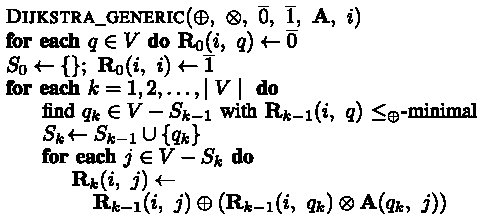
\includegraphics{algorithm.pdf}
% \caption{Dynerowicz and Griffin's imperative generalized Dijkstra's algorithm}
% \label{fig.algorithm}
% \end{figure}

\todo{finish me}

\paragraph{Agda}

Agda~\cite{norell_dependently_2009} is a dependently-typed programming language \emph{cum} proof assistant for higher-order intuitionistic logic.
In contrast to similar systems, such as Coq~\cite{bertot_short_2008} and Matita~\cite{asperti_matita_2011}, proof terms are constructed by hand via a process of type-directed refinement, rather than being constructed via tactic-assisted metaprogramming.

Agda has a uniform syntax that should be familiar to Haskell programmers and users of other dependently-typed proof assistants.
One syntactic novelty is a flexible system of user-declared Unicode mixfix identifiers~\cite{danielsson_parsing_2011} with `holes' in an identifier being denoted by underscores.
We write \AgdaSymbol{(}\AgdaBound{x}~\AgdaSymbol{:}~\AgdaBound{A}\AgdaSymbol{)}~\AgdaSymbol{→}~\AgdaBound{B} for the dependent function space where \AgdaBound{x} may occur in \AgdaBound{B}, and write \AgdaBound{A}~\AgdaSymbol{→}~\AgdaBound{B} when \AgdaBound{x} does not occur in \AgdaBound{B} as is usual.
We enclose arguments to be inferred in braces, as in \AgdaSymbol{\{}\AgdaBound{x}~\AgdaSymbol{:}~\AgdaBound{A}\AgdaSymbol{\}}~\AgdaSymbol{→}~\AgdaBound{B}, sometimes making use of the shorthands \AgdaSymbol{∀}~\AgdaBound{x}~\AgdaSymbol{→}~\AgdaBound{B} and \AgdaSymbol{∀}~\AgdaSymbol{\{}\AgdaBound{x}\AgdaSymbol{\}}~\AgdaSymbol{→}~\AgdaBound{B} when types can be inferred.
We write \AgdaDatatype{Σ}~\AgdaBound{A}~\AgdaBound{B} for the dependent sum type whose first projection has type \AgdaBound{A}, and write \AgdaBound{A}~\AgdaDatatype{×}~\AgdaBound{B} when the second projection does not depend on the first, as is usual.
Dependent sums are constructed using the comma constructor: \AgdaBound{x}~\AgdaInductiveConstructor{,}~\AgdaBound{y}.
We sometimes write \AgdaFunction{∃}~\AgdaSymbol{λ}~\AgdaBound{x}~\AgdaSymbol{→}~\AgdaBound{P} for the dependent sum type when the type of the first projection can be inferred.
Propositional equality between two types is written \AgdaBound{A}~\AgdaDatatype{≡}~\AgdaBound{B} and has a single canonical inhabitant, \AgdaInductiveConstructor{refl}.
Lastly, we write \AgdaBound{A}~\AgdaDatatype{⊎}~\AgdaBound{B} for the disjoint union type with constructors \AgdaInductiveConstructor{inj₁} and \AgdaInductiveConstructor{inj₂} and \AgdaFunction{¬}~\AgdaBound{A} for constructive negation.
Agda is a predicative type theory with an infinite universe hierarchy, \AgdaPrimitiveType{Setᵢ}, with \AgdaPrimitiveType{Set} being identified with \AgdaPrimitiveType{Set₀}, the base universe in Agda's hierarchy.
Universe polymorphism is used extensively throughout our development, with explicit quantification over universe levels that will henceforth be ignored.

%\paragraph{Contributions and map of paper}
%\subsection{Map of Paper}
%\label{subsect.map.of.paper}
%In Section~\ref{sect.basic.definitions} we cover some definitions needed to define Dijkstra's algorithm and its correctness proof.
%In Section~\ref{sect.path.algebras.their.properties.and.models} we discuss `path algebras', a variety of algebraic structure central to our proof of correctness, also providing three models of path algebras to demonstrate that models exist and that path algebras are not categorical.
%In Section~\ref{sect.dijkstras.algorithm.and.its.correctness} we discuss the imperative Dijkstra algorithm, our functional implementation, and main body of the correctness proof leading up to our main theorem: Dijkstra's algorithm computes a right-local solution.
%In Section~\ref{sect.example} we demonstrate the algorithm in action with an example execution inside Agda.
%In Section~\ref{sect.conclusions} we conclude.


\section{Basic definitions}
\label{sect.basic.definitions}

\subsection{Matrices and graph nodes}
\label{subsect.matrices.and.graph.nodes}

\input{matrices.tex}

\subsection{Big sums}
\label{subsect.sums}

\input{sums.tex}

% Representation of algebraic structures as records
% Setoid, Equivalence

% Subset, Bigop, EstimateOrder

\subsection{Sorted vectors}
\label{subsect.sorted.vectors}

\input{sorted-vectors.tex}


\section{Sobrinho Algebras, their properties and models}
\label{sect.path.algebras.their.properties.and.models}

\begin{figure}[t]
\centering
\begin{tabular}{c||l@{\;\;\;}|l}
\textbf{Operation} & \textbf{Semiring} & \textbf{Sobrinho Algebra} \\
\midrule
\AgdaFunction{\_+\_} & Associative & Associative \\
                 & Commutative & Commutative \\
                 & Identity: \AgdaField{0\#} & Identity: \AgdaField{0\#} \\
                 & ---                      & Selective \\
                 & ---                      & Zero: \AgdaField{1\#} \\
\midrule
\AgdaFunction{\_*\_} & Associative & --- \\
                 & Identity: \AgdaField{1\#} & Left identity: \AgdaField{1\#} \\
                 & Zero: \AgdaField{0\#}     & --- \\
\midrule
\AgdaFunction{\_*\_} and \AgdaFunction{\_+\_} & \AgdaFunction{\_*\_} distributes over \AgdaFunction{\_+\_} &
                   \AgdaFunction{\_+\_} absorbs \AgdaFunction{\_*\_} \\
\bottomrule
\end{tabular}
\label{tab.path.algebra}
\vspace{6pt}
\caption{Comparing the algebraic properties of a Semiring and a Sobrinho Algebra.}
\label{fig.path.algebra}
\end{figure}

Fix a carrier set $S$ and an equivalence relation $\_{≈}\_$.
We call a binary operation on $S$ \emph{selective} whenever $x \bullet y ≈ x$ or $x \bullet y ≈ y$ for any $x$ and $y$.
Intuitively, a selective binary operation denotes a `choice' between any two elements.
With this definition in mind, we call a 6-tuple $\langle S, \_{≈}\_, \_{+}\_, \_{*}\_, 0, 1 \rangle$ a `Sobrinho Algebra' whenever:
\begin{itemize}
\item
$\langle S, \_{≈}\_, \_{+}\_, 0 \rangle$ forms a commutative monoid,
\item
$1$ is a left identity for multiplication, and a left- and right zero for addition,
\item
Addition is selective, and addition absorbs multiplication,
\item
The usual closure and congruence properties for the unit elements and operations apply.
\end{itemize}
In Figure~\ref{fig.path.algebra}, we provide a comparison between the operations and laws of a Sobrinho Algebra and the more familiar notion of a Semiring, algebraic structures themselves often used in work on algebraic routing.

Following established convention, we capture the notion of a Sobrinho Algebra as an Agda record named \AgdaRecord{SobrinhoAlgebra}.
We call the carrier type, corresponding to the carrier set $S$ above, of a Sobrinho Algebra, \AgdaField{Carrier}, obtaining the closure properties mentioned above for `free' as a side-effect of Agda's typing discipline, and assume that there exists a decidable setoid equivalence relation on elements of this type, \AgdaField{\_≈\_}.
We use the names \AgdaField{1\#} and \AgdaField{0\#} for our two identity elements of the algebra within Agda, in order to avoid clashing with Agda's in-built numeral parsing notation for natural numbers.


\paragraph{Models}
\label{subsect.models}

\input{path-models.tex}

\paragraph{Properties}
\label{subsect.properties}

\input{path-properties.tex}

\section{Dijkstra's Algorithm and its correctness}
\label{sect.dijkstras.algorithm.and.its.correctness}

\input{dijkstra-impl.tex}

\paragraph{Correctness}
\label{subsect.correctness}

\input{dijkstra-correct.tex}

\section{Example}
\label{sect.example}

\input{example.tex}

\section{Conclusions}
\label{sect.conclusions}

In this paper we have presented a purely functional implementation of a generalised shortest path algorithm, and proved it correct.
We have made extensive use of dependent types, and some of Agda's more advanced features, such as induction-recursion, to help structure the implementation and proof.

\paragraph{Related Work}
Remarkably, despite the algorithm being well-known, Chen seems to have been the first to verify the correctness of Dijkstra's Algorithm in any proof assistant, when he produced a Mizar implementation in 2003~\cite{chen:dijkstra:2003}.
Later, Moore and Zhang verified Dijkstra's Algorithm in ACL2~\cite{moore:proof-pearl:2005}.
Gordon, Hurd, and Slind verified Dijkstra's reachability algorithm in HOL4 as part of a wider formalisation of the Accellera Property Specification Language~\cite{gordon:executing:2003}.
Fleury verified Floyd's all-pairs shortest path algorithm in Coq~\cite{fleury:implantation:1990}, and in unpublished work, Paulin and Fill\^iatre later verified Floyd's algorithm again in imperative form with the aid of an additional tool, also in Coq.
Nordhoff and Lammich verified Dijkstra's algorithm in Isabelle/HOL as a showcase of the Isabelle refinement and collections frameworks~\cite{nordhoff-dijkstra-2012}.
Lammich also later implemented and verified an imperative version of Dijkstra's Algorithm in Isabelle~\cite{lammich:refinement:2015}.
All of these prior formalisations take a very concrete, very classical approach to shortest path algorithms and their proofs of correctness, largely following textbook treatments, in contrast to our work presented in this paper.
In particular, we believe that we are the first to present a verified implementation of a shortest path algorithm employing the algebraic method.
%\todo{talk about equilibrium routing, etc. and relationship to this work}

The idea that Dijkstra's algorithm can be generalised to an algorithm that solves a matrix fixpoint equation was first explored by Sobrinho~\cite{sobrinho_algebra_2001}, with Mohri later presenting a general semiring framework for shortest path algorithms~\cite{mohri:semiring:2002} where the underlying semiring and queing discipline used by the algorithm are abstracted over, with Dijkstra being a special case.
Griffin and Sobrinho explored the solutions found by the generalised algorithm whenever distributivity is not assumed~\cite{sobrinho_routing_2010}.
Our work builds on these latter ideas, but goes beyond it in several ways: we specify the properties of the algebraic structure assumed, give a concrete implementation of the algorithm, and mechanically verify its correctness.

All implementation files, and supporting documentation, are available anonymously from a public \texttt{git} repository~\cite{markert_formalised_2015}.
The formalisation consists of approximately 2,400 lines of Agda and was developed using Agda~2.4.2.1 and~2.4.2.2 and Standard Library version~0.9.

We thank Timothy G.~Griffin for helpful comments when preparing this paper.
The second author is employed on EPSRC grant EP/K008528.


\bibliography{path-algebra}

\end{document}
